During the offline simulation and the initial real-time simulation cases, the fuzzy logic controller is designed using the MathWorks fuzzy logic toolbox \cite{WinNT6}. But to implement the FL controller in FPGA, VHDL (Very high speed integrated circuit Hardware Description Language) code is used as the Matlab HDL (Hardware description language) coder does not generate the automatic VHDL code for the fuzzy logic controller, the FL controller is designed from teh scratch. The FL controller has three major parts: 1) Fuzzification, 2) Inference and 3) Defuzzification.

\subsubsection{Fuzzification}
In this part, the membership functions of the input and output variables are defined. The membership function shapes are typically triangular, trapezoidal, Gaussian, and bell shaped. Fuzzy crisp input values are converted into membership values in the interval [0 1]. In fuzzification, the degree of membership is determined by locating the input in the membership function. The designed FL controller has four input variables ($\Delta I$, $V_{Bus}$, $SOC_{Bat}$, and $SOC_{SC}$) and one output variable ($P_{stor-ref}$). The membership functions of the input and output variables are shown in Fig. \ref{sec3_f4}. The first input variables, $\Delta I$ has three membership functions (Positive, Negative, Zero) and all of them are trapezoidal shaped. Fig. \ref{sec4_f6} shows a trapezoidal shaped membership function. The trapezoidal shaped membership function is divided into five regions. As a function of x, the five regions of the trapezoidal shaped membership function is represented in (\ref{equation-2}). Where x represents the crisp values of the input variables, y represents the degree of membership ($\mu$) and $a$, $b$, $c$, $d$ are four scalar parameters which define the shape of the trapezoidal membership function \cite{anand2012design}.
\begin{figure}[ht!]
\centering
%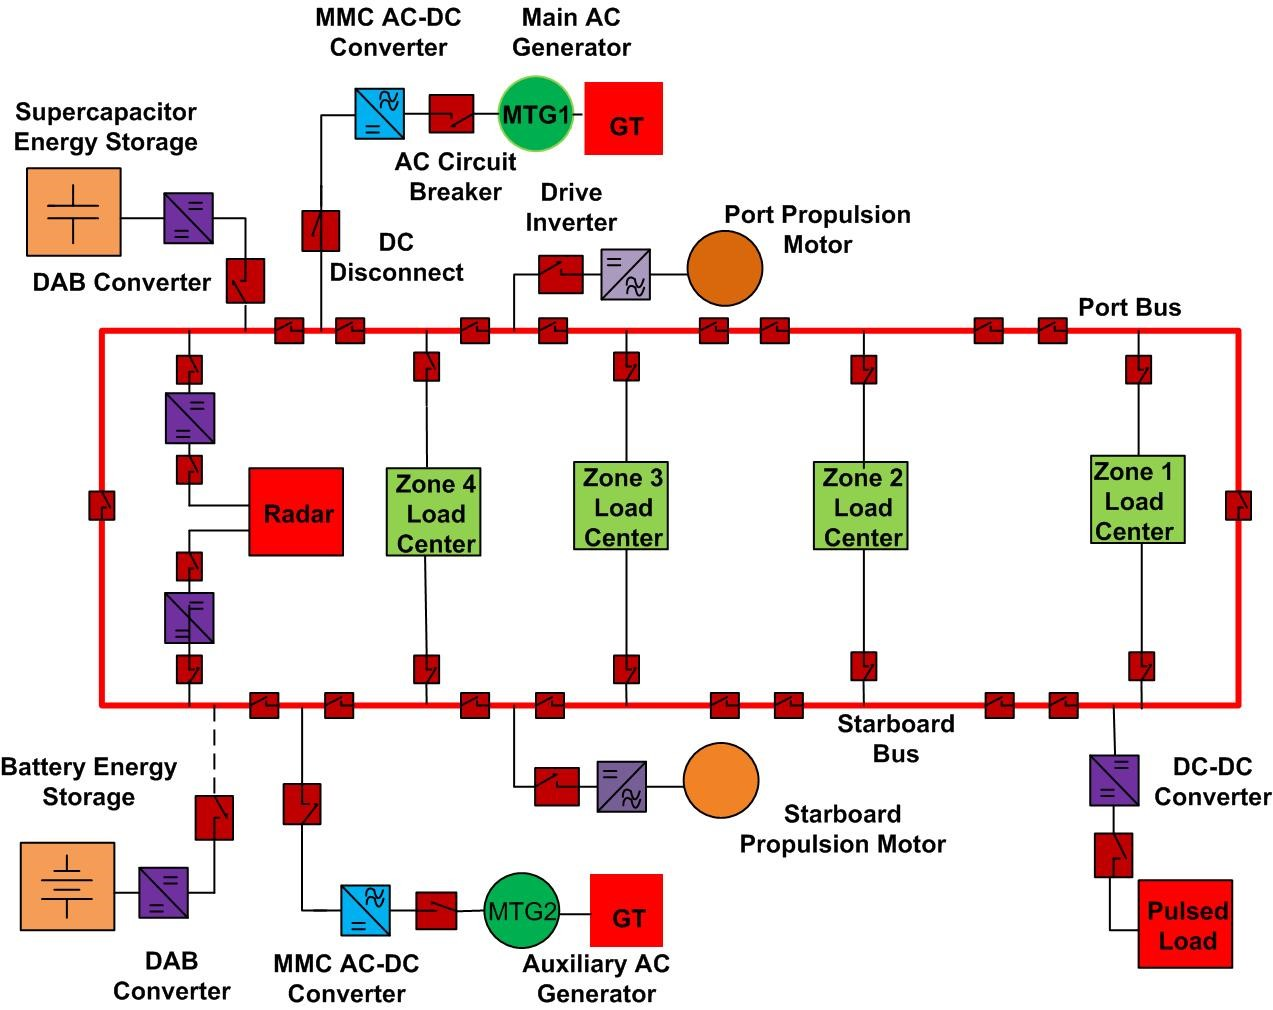
\includegraphics[width=\columnwidth]{f1}
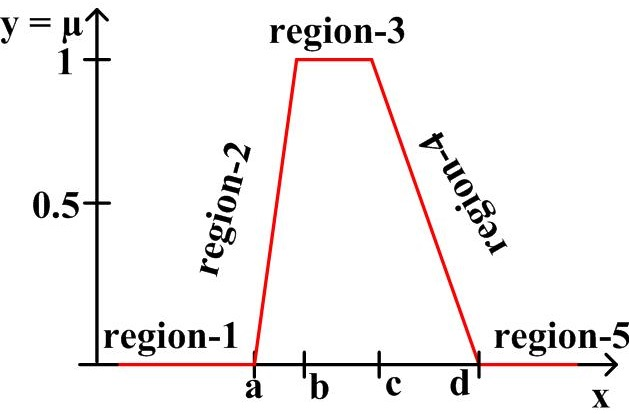
\includegraphics[width=2.0in, height=1.3in]{f6}
\caption{Trapezoidal-shaped membership functions.}
\label{sec4_f6}
\end{figure} 
\begin{equation}\label{equation-2}
f(x;a,b,c,d)=
    \begin{cases}
      0, &  x\leq a\\
      \frac{x-a}{b-a}, & a\leq x \leq b \\
       1, & b\leq x \leq c \\
       \frac{d-x}{d-c}, & c\leq x \leq d \\
       0, &  d\leq x
    \end{cases}
\end{equation}
For example, the Zero membership function of $\Delta I$ is represented in (\ref{equation-3}) where the values are $a$ = -720, $b$ = -40, $c$ = 40, and $d$ = 720. Similarly the other two membership functions (Negative and Positive) are represented. 

\begin{equation}\label{equation-3}
f(x;a,b,c,d)=
    \begin{cases}
      0, &  x\leq -720\\
      \frac{x-(-720)}{(-40)-(-720)}, & -720\leq x \leq -40 \\
       1, & -40\leq x \leq 40 \\
       \frac{720-x}{720-40}, & 40\leq x \leq 720 \\
       0, &  720\leq x
    \end{cases}
\end{equation}
The second input variables, $V_{Bus}$ has three membership functions (High, Low and Good). The Low and High membership function are trapezoidal shaped and they are designed as the similar way shown for the input variable $\Delta I$. The Good membership function is triangular shaped and it is divided into four regions. Fig. \ref{sec4_f7} shows a triangular shaped membership function. As a function of x, the four regions of the triangular shaped membership function is represented in (\ref{equation-4}). Where x represents the crisp values of the input variables, y represents the degree of membership ($\mu$) and $a$, $b$, and $c$ are three scalar parameters which define the shape of the triangularly shaped membership function. The Good membership function of the input variable, $V_{Bus}$ is triangular shaped, where the values are $a$ = 4940, $b$ = 5000, and $c$ = 5060. The third and fourth input variables ($SOC_{Bat}$, and $SOC_{SC}$) have three trapezoidal shaped membership functions and they are designed as the similar way shown in (\ref{equation-2}). The output variable, $P_{stor-ref}$ has two trapezoidal shaped membership functions (Negative, Positive), they are designed as the similar way shown in (\ref{equation-2}), one triangular shaped membership function (Zero) and it is designed as the similar way as shown in (\ref{equation-4}). 
\begin{figure}[ht!]
\centering
%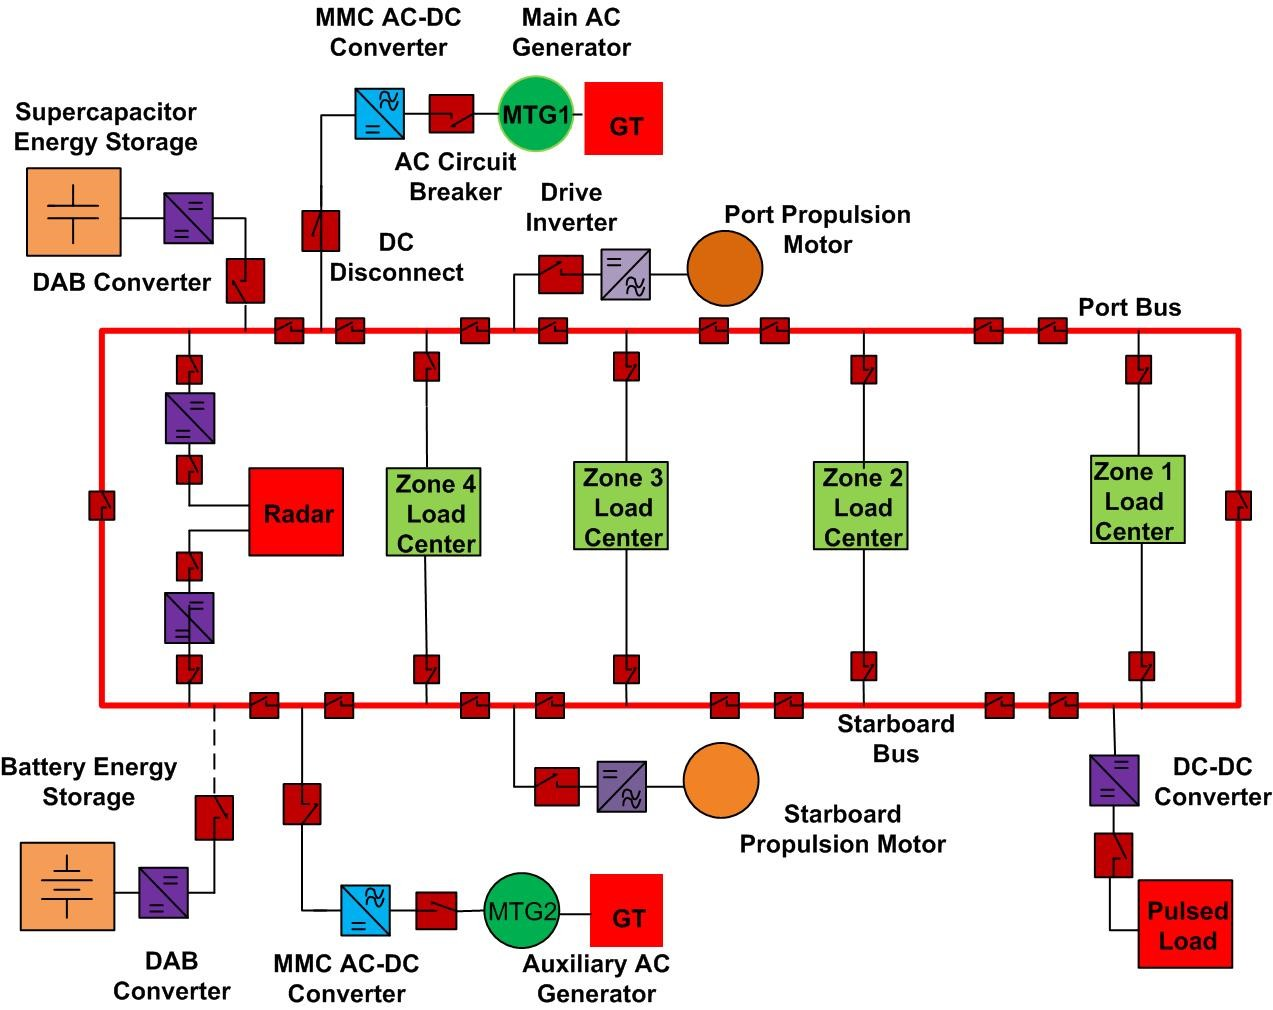
\includegraphics[width=\columnwidth]{f1}
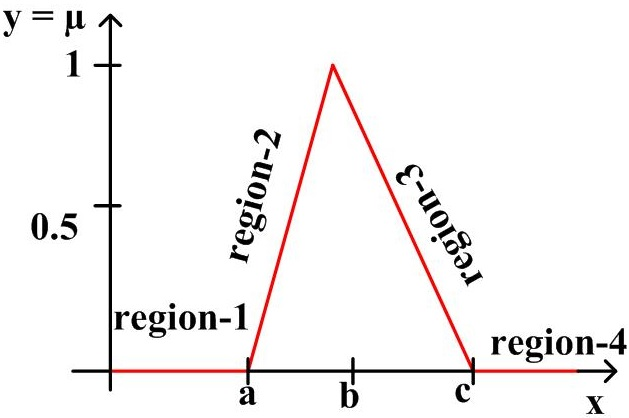
\includegraphics[width=2.0in, height=1.3in]{f7}
\caption{Triangular-shaped membership functions.}
\label{sec4_f7}
\end{figure}
\begin{equation}\label{equation-4}
f(x;a,b,c)=
    \begin{cases}
      0, &  x\leq a\\
      \frac{x-a}{b-a}, & a\leq x \leq b \\
       \frac{c-x}{c-b}, & b\leq x \leq c \\
       0, &  c\leq x
    \end{cases}
\end{equation}
\subsubsection{Inference}Fuzzy rules create the relationship between the output domain fuzzy sets and the input domain fuzzy sets. A fuzzy inference system makes fuzzy decisions based on fuzzy inputs and rules. The two common fuzzy operators for multiples antecedents are “fuzzy intersection or conjunction or minimum (AND)” and “fuzzy union or disjunction or maximum (OR)”. The fuzzy rules are shown in Table I and the first fuzzy rule is written in section III. For example, in a certain moment, the FL controller receives $\Delta I$ = -1000A, $V_{Bus}$ = 4400V, $SOC_{Bat}$ = 20\%, and $SOC_{SC}$ = 25\% as the inputs. After using the designed membership functions for the input variables, the degree of membership ($\mu$) of the input variables are  $\mu_{Negative}(\Delta I) = 1$, $\mu_{Low}(V_{Bus}) = 1$,  $\mu_{Low}(SOC_{Bat}) = 1$, and  $\mu_{Low}(SOC_{SC}) = 1$. According to first fuzzy rule, the degree of membership function, Zero of the output variable, $P_{stor-ref}$ is given in (\ref{equation-5})
\begin{multline}\label{equation-5}
\mu_{Zero}(P_{stor-ref})= min[(\mu_{Negative}(\Delta I), \mu_{Low}(V_{Bus}), \\
\mu_{Low}(SOC_{Bat}), \mu_{Low}(SOC_{Bat})]
\end{multline}
\subsubsection{Defuzzification} In defuzzification process, the degree of membership functions ($\mu$) of the output variable ($(P_{stor-ref}$) is converted to the actual crisp value. For defuzzification, the center of sums method is used \cite{ross2009fuzzy}. This method is similar to the weighted average method and it is faster than the many commonly used defuzzification methods. The output defuzzified crisp value ($z^{\ast}$) is calculated by using (\ref{equation-6}).  Here, $C_k(z)$ is the output fuzzy set and  $\bar{z}$ denotes the distance to the centroid of each of the respective membership functions. 
\begin{equation}\label{equation-6}
z^{\ast}=\frac{\sum_{k=1}^{n}\mu C_k(z)\int_z \bar{z} dz}{\sum_{k=1}^{n}\mu C_k(z)\int_z dz}
\end{equation}
\subsubsection{Implementation of CHIL on FPGA}
For CHIL implementation the ‘Xilinx Virtex-7 FPGA VC707 Evaluation Kit’ which is available with the OP7200 FPGA. The fuzzy logic controller has a very wide range of numbers. The degrees of membership need to be kept accurate to at least three decimal places to operate the FL controller properly. The numerator part of (\ref{equation-6}) can be in the range of $1 \times 10^{18}$.To accommodate this huge range with fixed point numbers at least 69 bits are necessary. The Xilinx vartex-7 FPGA running at 100MHz was not able to complete basic 69-bit arithmetic operations within in the allocated time (10ns).  For this reason the IEEE 754 single precision floating point number format \cite{sites2008ieee} is used for all the calculations. The floating point arithmetic functions for the VHDL code are generated using the Xilinx ‘LogiCORE IP Floating-Point Operator v5.0’ product. The rest of the system is designed using system generator, digital signal processor (DSP) provided by Xilinx.

Fig. \ref{sec4_f8} shows the model built with RT-XSG and Xilinx system generator blocks which are used to generate the final bit stream. As seen in the figure the $\Delta I, V_{bus}, SOC_{BAT} and SOC_{SC}$ signals are first converted from double to single precision floating point number  and then sent from the real time simulator to the FPGA running the FL algorithm. The fuzzification process uses the values of the signals sent from the simulator to generate the membership values. Then these values are used in the defuzzification and inference process to generate the power reference needed for the energy storage. The generated power reference is then sent to the simulator and converted back to double precision floating point number and used for the simulation.   
\begin{figure}[ht!]
\centering
%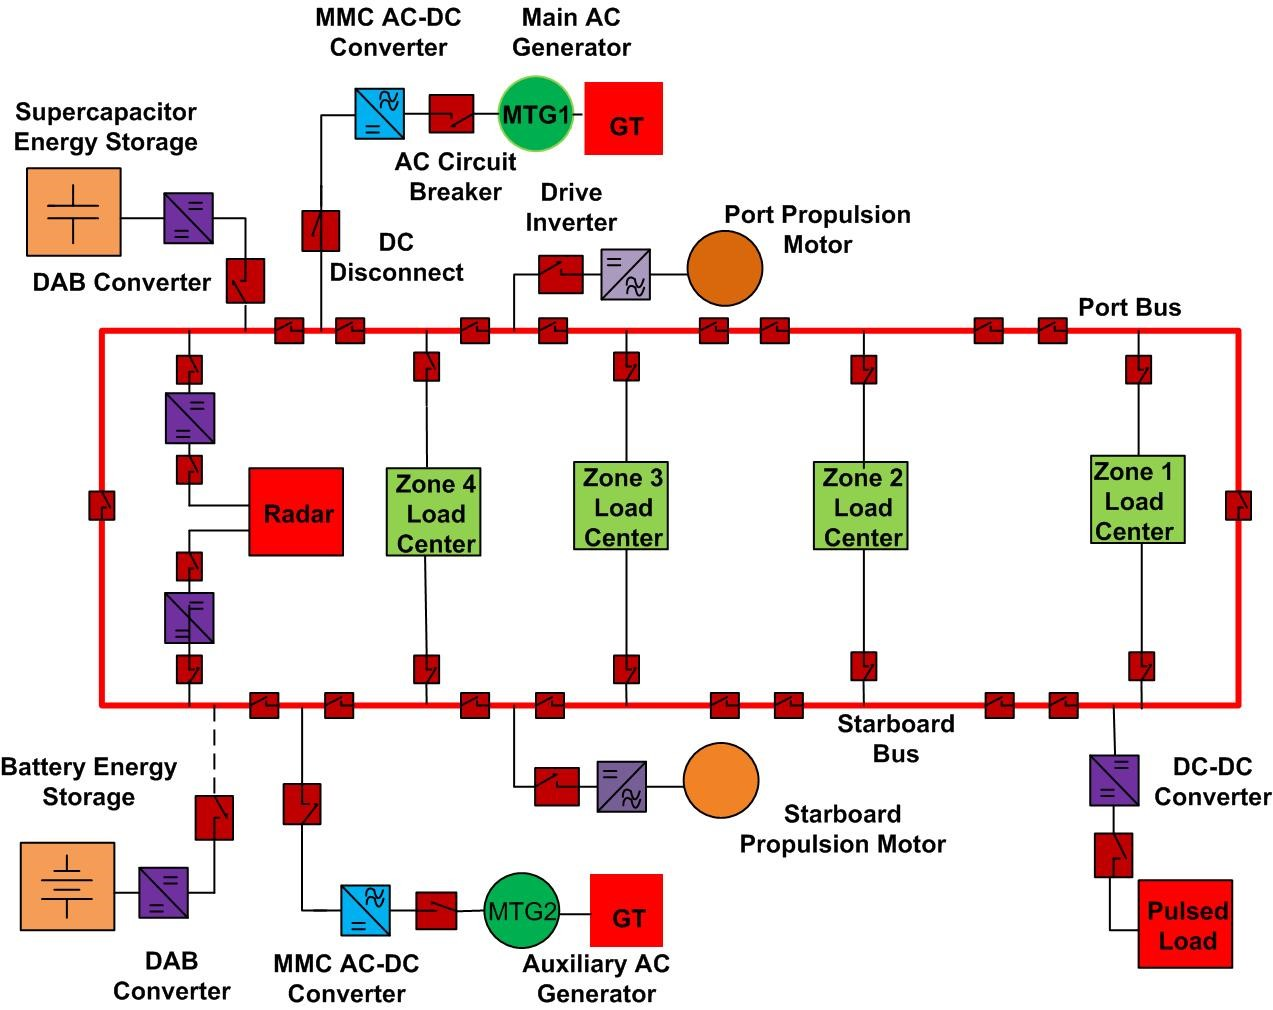
\includegraphics[width=\columnwidth]{f1}
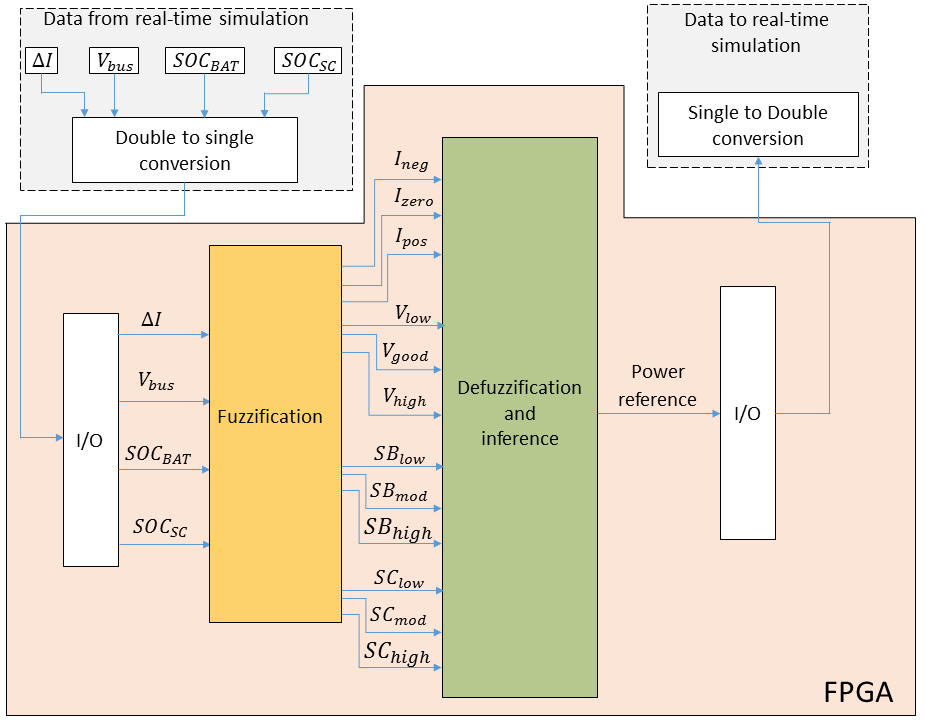
\includegraphics[width=3.5in]{f8}
\caption{Xilinx system generator model.}
\label{sec4_f8}
\end{figure}

Fig. \ref{sec4_f9} shows the implementation of one of the 81 rules derived from Table 1. From Fig. \ref{sec4_f9}, in the black box, the minimum value of all degrees of memberships is determined for a single rule. The output of this part is the $\mu_{Zero}(P_{stor-ref})$ according to (\ref{equation-5}). In the dotted box, the individual numerator ('A') and denominator ('B') component of (\ref{equation-6}) are determined for that respective rule. From Fig. \ref{sec4_f9}, the output ‘A’ represents the individual numerator component of (\ref{equation-6}) and the output ‘B’ represents the individual denominator component of (\ref{equation-6}) for a single rule. Finally, all the numerator ('A') components are summed and all the denominator ('B') components are summed individually for all the rules. Eventually, the sum of numerator components is divided by the sum of the denominator components according to (\ref{equation-6}) to generate the crisp output value ($P_{stor-ref}$). 
\begin{figure}[ht!]
\centering
%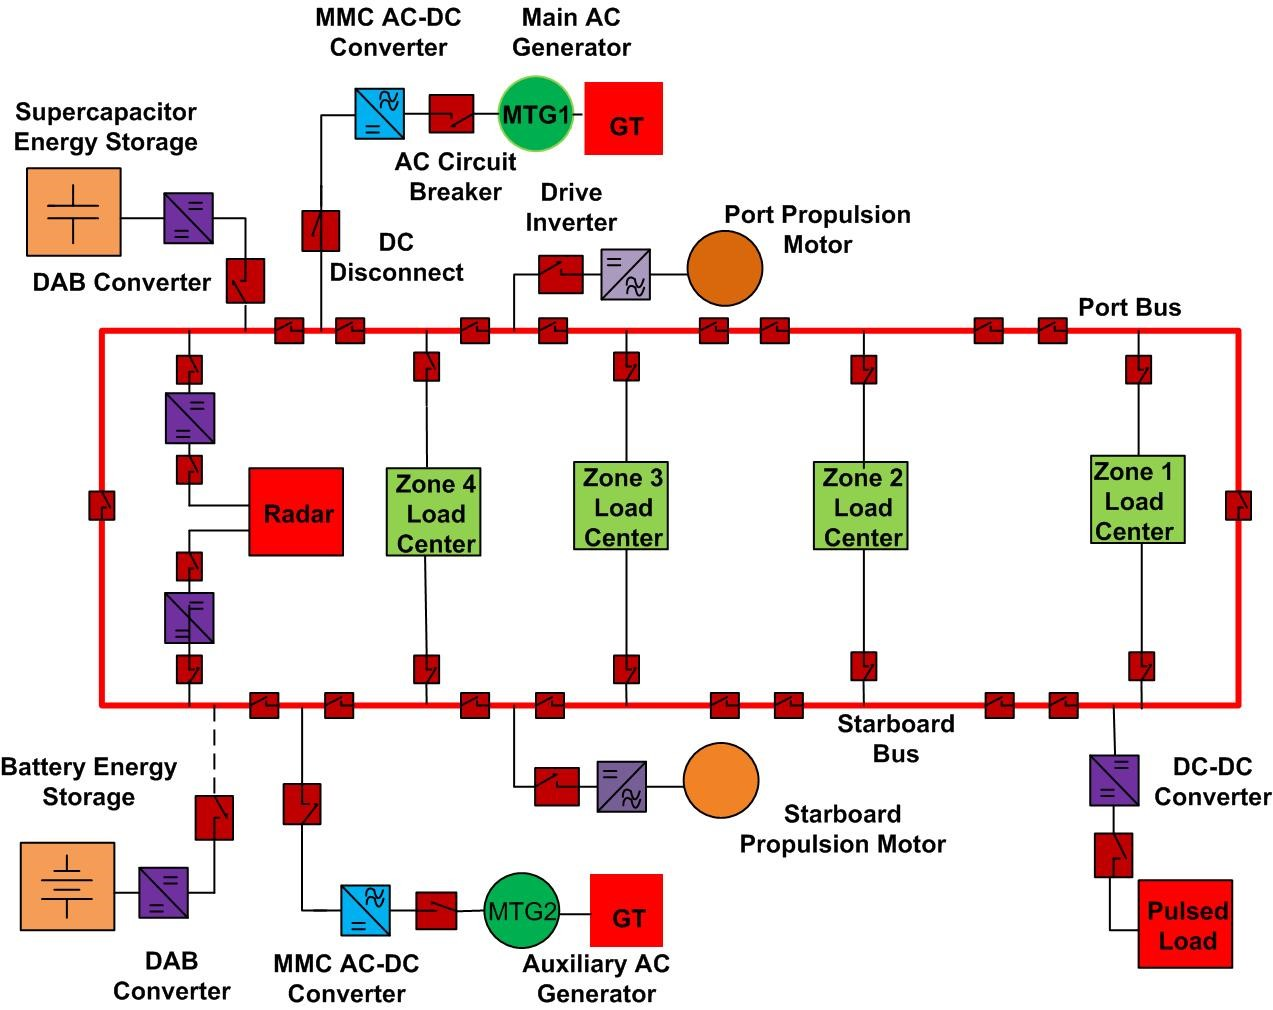
\includegraphics[width=\columnwidth]{f1}
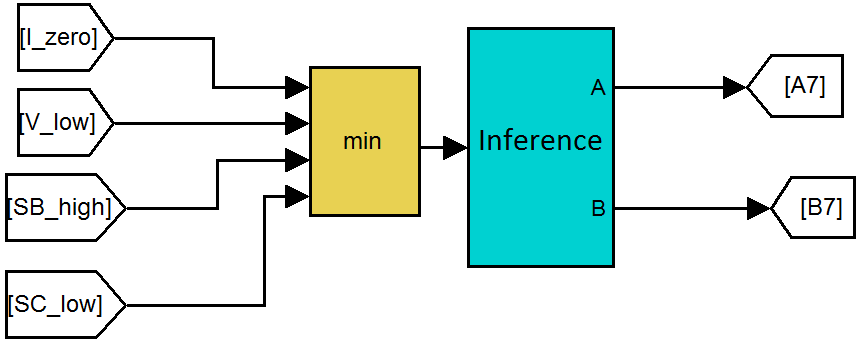
\includegraphics[width=3.5in]{f9}
\caption{Implementation of inference and defuzzification.}
\label{sec4_f9}
\end{figure}
